\documentclass[9pt]{beamer}
\mode<presentation>

% Theme choice:
\usetheme{Madrid}%Darmstadt 
\usepackage{xcolor}
\definecolor{mGreen}{rgb}{0,0.6,0}
\definecolor{mRed}{rgb}{0.6,0,0}
\usecolortheme[RGB={0,100,50}]{structure}
 \usefonttheme{structurebold} 
\setbeamercovered{invisible}
%\setbeamertemplate{navigation symbols}{}
\usepackage{dynblocks}
\usepackage{textpos}
\usepackage{amsfonts}
\usepackage{amsmath}
\usepackage{amssymb}
\usepackage{amsthm}
\usepackage{listings}
\usepackage{tikz}
\usepackage{pgfplots}
\pgfplotsset{compat=1.18}
\newtheorem{teorema}{Teorema}\usepackage{mathtools}
\renewcommand{\proofname}{Prova}
\usepackage[portuguese]{babel}

\uselanguage{Portuguese}
\languagepath{Portuguese}

\deftranslation[to=Portuguese]{Theorem}{Teorema}
\deftranslation[to=Portuguese]{Lemma}{Lema}
\deftranslation[to=Portuguese]{Corollary}{Corolário}
\deftranslation[to=Portuguese]{Proof}{Prova}

\usepackage{dutchcal}
\usepackage{hyperref}
\usepackage[utf8]{inputenc}
\usepackage[T1]{fontenc}
\usepackage{amsthm}


\usepackage[affil-it]{authblk} 
\usepackage{etoolbox}
\usepackage{lmodern}

\makeatletter
\patchcmd{\@maketitle}{\LARGE \@title}{\fontsize{18}{19.2}\selectfont\@title}{}{}
\makeatother

\renewcommand\Authfont{\fontsize{12}{14.4}\selectfont}
\renewcommand\Affilfont{\fontsize{9}{10.8}\itshape}

% Title page details: 
\title[Presentation]{DevOps e Site Reliability Engineering} %add title


\institute[UniRV]{\textbf{\large  \textcolor{structure}{\textbf{\large
Processo de Software
}} %add name 
% \hspace{0.5pt}
\\ \qquad
\\Professor: Me. Sergio Souza Novak 
\\Faculdade de Engenharia de Software}
} 
% \titlegraphic{\includegraphics[width=5cm]{msu.eps}}
\titlegraphic{
\includegraphics[width=5cm]{Universidade_de_Rio_Verde.jpg}}
\date{}

% Logo only on title page
%\logo{
\includegraphics[width=1cm,keepaspectratio]{Logo.png}}
\usepackage[pscoord]{eso-pic}

% TikZ libraries
\usetikzlibrary{shapes.geometric, shapes.symbols, arrows.meta, positioning, calc, fit, backgrounds, decorations.pathreplacing, shadows.blur}

\begin{document}

% Title page frame1
    %\titlepage 
%\end{frame}
\frame[plain]{\titlepage}
%logo
\AddToShipoutPictureFG{
    \put(\LenToUnit{.92\paperwidth},
    \LenToUnit{.185\paperheight})
    {\vtop{{\null}
    \makebox{
\includegraphics[width=.8cm,keepaspectratio]{Universidade_de_Rio_Verde.jpg}}}}}
 
% ----------------------------------------------------------
% Slide: Referência Bibliográfica
% ----------------------------------------------------------
\begin{frame}{Referência Bibliográfica Principal} 
\begin{columns}[c]
  \begin{column}{0.38\textwidth}
    \begin{center}
      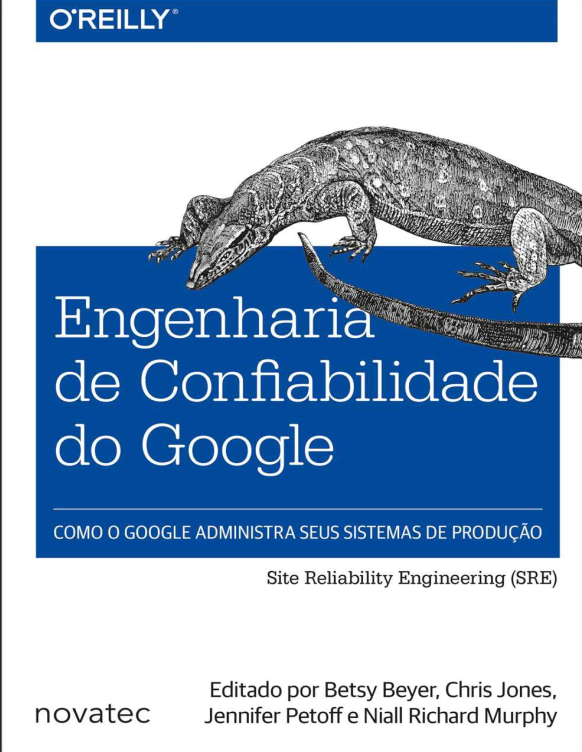
\includegraphics[width=0.85\textwidth,keepaspectratio]{livro.png}
    \end{center}
  \end{column}
  \begin{column}{0.60\textwidth}
    \begin{block}{Livro Base da Aula}
      \textbf{Site Reliability Engineering}\\
      \textit{How Google Runs Production Systems}
    \end{block}
    
    \vspace{0.15cm}
    \begin{itemize}
      \item \textbf{Autores:} Betsy Beyer, Chris Jones, Jennifer Petoff \& Niall Richard Murphy
      \item \textbf{Editora:} O'Reilly Media / Google SRE
      \item \textbf{Foco:} Engenharia de Confiabilidade de Sistemas, automação, cultura sem culpa e gerenciamento de incidentes em escala global. 
    \end{itemize}
  \end{column}
\end{columns}
\end{frame}

\begin{frame}{Sumário}
  \begin{columns}[t]
    \begin{column}{0.48\textwidth}
      \tableofcontents[sections={1-4}]
    \end{column}
    \hfill
    \begin{column}{0.48\textwidth}
      \tableofcontents[sections={5-8}]
    \end{column}
  \end{columns}
\end{frame}

% ============================================================
% SEÇÃO 1: Abordagem Tradicional com Administradores de Sistemas
% ============================================================
\section{Abordagem Tradicional com Sysadmins}

\subsection{Conceitos Preliminares}

% ----------------------------------------------------------
% Slide: O que é um Pager?
% ----------------------------------------------------------
\begin{frame}[fragile]{Conceito Fundamental: O que é um Pager?}
\begin{block}{Definição e Origem}
Historicamente, o \textbf{pager} (ou bip) era um pequeno dispositivo físico de bolso que emitia um sinal sonoro estridente quando uma emergência ocorria. Hoje, em SRE, o termo refere-se ao \textbf{sistema de alerta de emergência crítica}.
\end{block}

\vspace{0.15cm}
\begin{center}
\begin{tikzpicture}[
    box/.style={draw, rounded corners=6pt, thick, minimum width=2.1cm, minimum height=0.9cm, font=\tiny\bfseries, align=center},
    arr/.style={-{Stealth[length=5pt]}, thick, structure!70},
]
    % --- Desenho do Dispositivo Pager ---
    \draw[fill=gray!80!black, rounded corners=8pt, thick] (-4.5, 0.9) rectangle (-2.3, -1.1);
    % Tela do Pager
    \fill[green!25!black, rounded corners=3pt] (-4.3, 0.2) rectangle (-2.5, 0.7);
    \node[font=\tiny\ttfamily, green!80!lightgray] at (-3.4, 0.45) {ALERTA: DB DOWN!};
    % Botão do Pager
    \fill[red!70] (-2.7, -0.6) circle (0.15);
    \node[font=\tiny, white] at (-2.7, -0.6) {BIP};
    \fill[gray!40] (-3.8, -0.6) rectangle (-3.2, -0.4);
    \node[font=\tiny\bfseries, white] at (-3.4, -1.3) {Pager Físico (Bip)};

    % --- Fluxo de Alerta Moderno ---
    \node[box, fill=red!15] (mon) at (-0.8, 0.5) {Monitoramento\\(Prometheus/Grafana)};
    \node[box, fill=orange!15] (sys) at (1.6, 0.5) {Sistema de Pager\\(PagerDuty/Opsgenie)};
    \node[box, fill=green!15] (eng) at (4.0, 0.5) {Engenheiro de\\Plantão (On-Call)};

    \draw[arr] (mon) -- node[above, font=\tiny] {Falha Crítica} (sys);
    \draw[arr] (sys) -- node[above, font=\tiny] {Notificação 24/7} (eng);

    \node[draw=structure!50, rounded corners=4pt, fill=structure!10, font=\tiny, text width=5.8cm, align=center] at (1.6, -0.7) {\textbf{Regra de Ouro}: O Pager só deve tocar quando um \textbf{ser humano} precisa tomar uma ação \textbf{imediata} em produção!};
\end{tikzpicture}
\end{center}

\vspace{0.1cm}
\begin{exampleblock}{\scriptsize Aplicação no Dia a Dia}
Estar ``on-call'' (de plantão) significa carregar o pager: se o sistema cair às 3h da manhã, o pager toca e o engenheiro deve acordar para resolver o incidente.
\end{exampleblock}
\end{frame}

\subsection{Contexto Histórico e Processo}

% ----------------------------------------------------------
% Slide 1: Contexto Histórico
% ----------------------------------------------------------
\begin{frame}{Contexto Histórico}
\begin{block}{Como as empresas operavam seus sistemas?}
Historicamente, as empresas empregaram \textbf{administradores de sistemas} (sysadmins) para operar sistemas computacionais complexos.
\end{block}

\vspace{0.3cm}
\begin{center}
\begin{tikzpicture}[
    box/.style={draw, rounded corners, fill=structure!15, minimum width=2.2cm, minimum height=0.9cm, align=center, font=\scriptsize\bfseries},
    arr/.style={-{Stealth[length=3mm]}, thick, structure!70},
]
    \node[box] (comp1) at (0,0) {Componente\\de Software A};
    \node[box] (comp2) at (3,0) {Componente\\de Software B};
    \node[box] (comp3) at (6,0) {Componente\\de Software C};
    
    \node[box, fill=orange!20, minimum width=7.5cm] (sysadmin) at (3,-1.8) {\large Sysadmin integra e opera o serviço};
    
    \node[box, fill=blue!15, minimum width=7.5cm] (servico) at (3,-3.3) {\large Serviço em Produção};
    
    \draw[arr] (comp1.south) -- (sysadmin.north -| comp1);
    \draw[arr] (comp2.south) -- (sysadmin.north);
    \draw[arr] (comp3.south) -- (sysadmin.north -| comp3);
    \draw[arr] (sysadmin.south) -- (servico.north);
\end{tikzpicture}
\end{center}
\end{frame}

% ----------------------------------------------------------
% Slide 1.1: Estudo de Caso (Sistema de E-Commerce)
% ----------------------------------------------------------
\begin{frame}[fragile]{Estudo de Caso: E-Commerce Tradicional}
\begin{exampleblock}{Cenário Real: Lançamento de Nova Versão da Loja Virtual}
Como o fluxo tradicional funcionava na prática para uma aplicação web com banco de dados?
\end{exampleblock}

\vspace{0.2cm}
\begin{center}
\begin{tikzpicture}[
    box/.style={draw, rounded corners=6pt, thick, minimum width=2.2cm, minimum height=0.9cm, font=\tiny\bfseries, align=center},
    arr/.style={-{Stealth[length=3mm]}, thick, structure!70},
]
    % Devs
    \node[box, fill=blue!10] (dev) at (-3.8, 1.2) {Devs criam código\\(Loja, Cartão, estoque)};
    
    % Artifacts
    \node[box, fill=yellow!15] (pkg) at (0, 1.2) {Pacote ZIP / scripts\\enviados por e-mail/FTP};
    
    % Sysadmin manual work
    \node[box, fill=orange!20, minimum width=3.2cm] (sa) at (0, -0.6) {Sysadmin aciona SSH\\-- Configura Apache/Nginx\\-- Roda scripts SQL\\-- Atualiza dependências};

    % Production Server
    \node[box, fill=green!15, minimum width=3.2cm] (prod) at (4.2, -0.6) {Servidor de Produção\\(E-Commerce Online)};

    \draw[arr] (dev) -- (pkg);
    \draw[arr] (pkg) -- (sa);
    \draw[arr] (sa) -- (prod);
\end{tikzpicture}
\end{center}

\begin{block}{\scriptsize Fluxo Manual}
O Desenvolvedor entrega o pacote e o \textbf{Sysadmin assume total responsabilidade} por fazer o código funcionar no servidor de produção.
\end{block}
\end{frame}

% ----------------------------------------------------------
% Slide 1.2: Problemas do Processo Tradicional (Estudo de Caso)
% ----------------------------------------------------------
\begin{frame}[fragile]{Problemas do Processo Tradicional}
\begin{alertblock}{O que acontece em datas críticas (ex: Black Friday)?}
A dependência de intervenção humana em processos manuais gera falhas severas.
\end{alertblock}

\vspace{0.2cm}
\begin{center}
\begin{tikzpicture}[
    prob/.style={draw, rounded corners=6pt, fill=red!10, draw=red!40, thick, minimum width=3.8cm, minimum height=1.1cm, font=\tiny, align=center},
]
    \node[prob] (p1) at (-2.3, 1) {
        \textbf{Erro Humano em Scripts}\\
        Execução manual de SQL ou configs\\
        pode derrubar a loja em produção.
    };

    \node[prob] (p2) at (2.3, 1) {
        \textbf{Servidores ``Snowflake''}\\
        Apenas o Sysadmin conhece\\
        o estado exato da máquina.
    };

    \node[prob] (p3) at (-2.3, -0.6) {
        \textbf{Demora no Rollback}\\
        Se der erro, desfazer a atualização\\
        manual pode levar horas.
    };

    \node[prob] (p4) at (2.3, -0.6) {
        \textbf{Gargalo Operacional}\\
        Acúmulo de tarefas de deploy\\
        paralisa novas funcionalidades.
    };
\end{tikzpicture}
\end{center}
\end{frame}

\subsection{O Papel do Sysadmin e Escalabilidade}

% ----------------------------------------------------------
% Slide 2: Papel do Sysadmin
% ----------------------------------------------------------
\begin{frame}{O Papel do Administrador de Sistemas}
\begin{columns}[T]
\column{0.5\textwidth}
\begin{alertblock}{Responsabilidades}
\begin{itemize}
    \item Operar o serviço no dia a dia
    \item Responder a \textbf{eventos} (incidentes)
    \item Aplicar \textbf{atualizações} e mudanças
    \item Manter a infraestrutura estável
\end{itemize}
\end{alertblock}

\column{0.5\textwidth}
\begin{center}
\begin{tikzpicture}[
    icon/.style={circle, draw, thick, minimum size=1cm, fill=structure!10, font=\large},
    lbl/.style={font=\scriptsize, align=center},
]
    \node[icon] (admin) at (0,0) {\textbf{SA}};
    \node[lbl, below=2pt of admin] {Sysadmin};
    
    \node[icon, fill=red!15] (evt) at (2.2, 1.2) {!};
    \node[lbl, right=2pt of evt] {Eventos};
    
    \node[icon, fill=yellow!20] (upd) at (2.2, 0) {$\uparrow$};
    \node[lbl, right=2pt of upd] {Atualizações};
    
    \node[icon, fill=green!15] (ops) at (2.2, -1.2) {$\circlearrowleft$};
    \node[lbl, right=2pt of ops] {Operações};
    
    \draw[-{Stealth}, thick, red!60] (evt.west) -- (admin.east |- evt.west);
    \draw[-{Stealth}, thick, orange!70] (upd.west) -- (admin.east);
    \draw[-{Stealth}, thick, green!60!black] (ops.west) -- (admin.east |- ops.west);
\end{tikzpicture}
\end{center}
\end{columns}
\end{frame}

% ----------------------------------------------------------
% Slide 3: Escalabilidade do Modelo Sysadmin
% ----------------------------------------------------------
\begin{frame}{Escalabilidade do Modelo Tradicional}
\begin{exampleblock}{Problema Central}
À medida que a \textbf{complexidade} e o \textbf{volume de tráfego} aumentam, a equipe de sysadmins precisa crescer \textbf{proporcionalmente}.
\end{exampleblock}

\vspace{0.2cm}
\begin{center}
\begin{tikzpicture}
\begin{axis}[
    width=8cm, height=4.5cm,
    xlabel={Complexidade / Tráfego},
    ylabel={Tamanho da Equipe},
    xlabel style={font=\scriptsize},
    ylabel style={font=\scriptsize},
    tick label style={font=\tiny},
    xmin=0, xmax=10, ymin=0, ymax=10,
    axis lines=left,
    grid=major,
    grid style={gray!30},
    area style,
]
\addplot[thick, structure, fill=structure!15] coordinates {(0,0.5) (2,1.5) (4,3) (6,5) (8,7) (10,9.5)} \closedcycle;
\addlegendentry{\scriptsize Equipe de Sysadmins}
\end{axis}

\node[draw, rounded corners, fill=red!10, font=\scriptsize, align=center] at (7.5, 3.8) {Custo cresce\\linearmente!};
\end{tikzpicture}
\end{center}
\end{frame}

% ----------------------------------------------------------
% Slide 4: Separação Dev / Ops
% ----------------------------------------------------------
\begin{frame}[fragile]{A Separação Dev / Ops}
\begin{block}{Divisão Natural}
Como sysadmins e desenvolvedores têm \textbf{habilidades distintas}, são separados em equipes: \textbf{Desenvolvimento} e \textbf{Operações}.
\end{block}

\vspace{0.3cm}
\begin{center}
\begin{tikzpicture}[
    team/.style={draw, rounded corners, minimum width=3.5cm, minimum height=2.5cm, thick},
    member/.style={circle, draw, minimum size=0.5cm, inner sep=0},
    lbl/.style={font=\small\bfseries, align=center},
]
    % Dev team
    \node[team, fill=blue!5, draw=blue!60] (dev) at (0, 0) {};
    \node[lbl, blue!70] at (0, 1.6) {Desenvolvimento};
    \node[member, fill=blue!30] at (-0.8, 0.4) {};
    \node[member, fill=blue!30] at (0, 0.4) {};
    \node[member, fill=blue!30] at (0.8, 0.4) {};
    \node[font=\scriptsize, align=center] at (0, -0.5) {Novas funcionalidades\\Código do produto};
    
    % Ops team
    \node[team, fill=orange!5, draw=orange!60] (ops) at (5.5, 0) {};
    \node[lbl, orange!70!black] at (5.5, 1.6) {Operações (Ops)};
    \node[member, fill=orange!40] at (4.7, 0.4) {};
    \node[member, fill=orange!40] at (5.5, 0.4) {};
    \node[member, fill=orange!40] at (6.3, 0.4) {};
    \node[font=\scriptsize, align=center] at (5.5, -0.5) {Manter o serviço\\Responder incidentes};
    
    % Wall
    \draw[ultra thick, red!60, dashed] (2.75, -1.5) -- (2.75, 2.2);
    \node[font=\scriptsize\bfseries, red!60, rotate=90] at (2.75, 0.3) {SEPARAÇÃO};
\end{tikzpicture}
\end{center}
\end{frame}

% ============================================================
% SEÇÃO 2: Vantagens e Desvantagens
% ============================================================
\section{Vantagens e Desvantagens do Modelo Tradicional}

\subsection{Vantagens do Modelo Sysadmin}

% ----------------------------------------------------------
% Slide 5: Vantagens
% ----------------------------------------------------------
% ----------------------------------------------------------
% Slide 5: Visão Geral das Vantagens
% ----------------------------------------------------------
\begin{frame}[fragile]{Vantagens do Modelo Sysadmin: Visão Geral}
\begin{center}
\begin{tikzpicture}[
    adv/.style={draw, rounded corners=8pt, fill=green!10, thick, minimum width=5cm, minimum height=0.7cm, font=\scriptsize, align=center, drop shadow={shadow xshift=1pt, shadow yshift=-1pt, opacity=0.15}},
]
    \node[font=\small\bfseries, structure] at (0, 2.8) {Vantagens do Modelo Tradicional};
    
    \node[adv] (a1) at (0, 2.0) {\textbf{1. Fácil de implementar} — paradigma conhecido};
    \node[adv] (a2) at (0, 1.0) {\textbf{2. Muitos exemplos} disponíveis no mercado};
    \node[adv] (a3) at (0, 0.0) {\textbf{3. Talentos disponíveis} — profissionais prontos};
    \node[adv] (a4) at (0, -1.0) {\textbf{4. Ferramentas prontas} — softwares COTS e integradores};
    \node[adv] (a5) at (0, -2.0) {\textbf{5. Sem reinventar a roda} — infraestrutura existente};
    
    \foreach \i in {1,...,5} {
        \node[circle, fill=structure, text=white, font=\tiny\bfseries, inner sep=2pt] at (-3.2, {2.0-1.0*(\i-1)}) {\i};
    }
\end{tikzpicture}
\end{center}
\end{frame}

% ----------------------------------------------------------
% Slide 5.1: Vantagem 1 — Facilidade de Implementação
% ----------------------------------------------------------
\begin{frame}[fragile]{Vantagem 1: Facilidade de Implementação}
\begin{block}{Explicação Conceitual}
Por ser um paradigma estabelecido há décadas, a empresa não precisa reinventar papéis organizacionais. As tarefas de Ops são claras: montar servidores, instalar software e responder a incidentes.
\end{block}

\vspace{0.2cm}
\begin{exampleblock}{Estudo de Caso: Startup de Software SaaS (FinTechX)}
Uma startup de gestão financeira contrata \textbf{1 Sysadmin sênior}. Em poucas semanas, ele configura servidores Linux (Nginx + MySQL) em um provedor de nuvem tradicional. A empresa começa a operar rapidamente sem gastar meses desenhando processos complexos.
\end{exampleblock}

\vspace{0.2cm}
\begin{center}
\begin{tikzpicture}[
    nd/.style={draw, rounded corners=6pt, thick, minimum width=2.8cm, minimum height=0.7cm, font=\tiny\bfseries, align=center},
    arr/.style={-{Stealth}, thick, structure!60},
]
    \node[nd, fill=blue!10] (n1) at (0,0) {Contratar Sysadmin};
    \node[nd, fill=yellow!15] (n2) at (3.2,0) {Subir Servidor Padrão};
    \node[nd, fill=green!15] (n3) at (6.4,0) {Serviço no Air!};

    \draw[arr] (n1) -- (n2);
    \draw[arr] (n2) -- (n3);
\end{tikzpicture}
\end{center}
\end{frame}

% ----------------------------------------------------------
% Slide 5.2: Vantagem 2 — Abundância de Talentos
% ----------------------------------------------------------
\begin{frame}[fragile]{Vantagem 2: Abundância de Talentos no Mercado}
\begin{block}{Explicação Conceitual}
O mercado de trabalho possui um vasto grupo de profissionais formados com certificações e conhecimentos consolidados (Linux LPIC, Windows Server, Redes Cisco).
\end{block}

\vspace{0.2cm}
\begin{exampleblock}{Estudo de Caso: Empresa de Software RH (RHSoft)}
A \textit{RHSoft} precisa substituir um membro da equipe de operações. Ela abre uma vaga de "Administrador de Redes e Sistemas". Em poucos dias, recebe dezenas de currículos de profissionais já capacitados a operar seus servidores Apache e PostgreSQL, sem necessidade de treinamento intensivo.
\end{exampleblock}

\vspace{0.2cm}
\begin{center}
\begin{tikzpicture}[
    box/.style={draw, rounded corners=6pt, thick, minimum width=2.4cm, minimum height=0.8cm, font=\tiny\bfseries, align=center},
]
    \node[box, fill=orange!15] (b1) at (-2.8,0) {Vaga Tradicional\\de Sysadmin};
    \node[box, fill=green!15] (b2) at (0,0) {Amplo Banco de\\Candidatos};
    \node[box, fill=blue!15] (b3) at (2.8,0) {Contratação e\\Produtividade Rápida};

    \draw[-{Stealth}, thick] (b1) -- (b2);
    \draw[-{Stealth}, thick] (b2) -- (b3);
\end{tikzpicture}
\end{center}
\end{frame}

% ----------------------------------------------------------
% Slide 5.3: Vantagem 3 — Ferramentas Prontas (COTS)
% ----------------------------------------------------------
\begin{frame}[fragile]{Vantagem 3: Ferramentas Prontas e Integradores}
\begin{block}{Explicação Conceitual}
Existe um ecossistema maduro de softwares comerciais e open-source (Zabbix, Nagios, cPanel, VMware), além de consultorias terceirizadas de TI prontas para ajudar.
\end{block}

\vspace{0.2cm}
\begin{exampleblock}{Estudo de Caso: ERP Médico (MedApp)}
A empresa desenvolvedora do \textit{MedApp} prefere focar 100\% do seu time de dev na criação de funcionalidades médicas. Em vez de desenvolver um sistema próprio de monitoramento, ela instala o \textbf{Zabbix} e contrata uma consultoria de TI local para gerenciar os backups diários.
\end{exampleblock}

\vspace{0.2cm}
\begin{center}
\begin{tikzpicture}[
    tool/.style={draw, rounded corners=4pt, fill=structure!15, font=\tiny\bfseries, minimum width=1.8cm, minimum height=0.6cm, align=center},
]
    \node[tool] at (-3,0) {Zabbix / Nagios\\(Monitoramento)};
    \node[tool] at (0,0) {VMware / cPanel\\(Gestão)};
    \node[tool] at (3,0) {Consultorias TI\\(Suporte Terceirizado)};
\end{tikzpicture}
\end{center}
\end{frame}

% ----------------------------------------------------------
% Slide 5.4: Vantagem 4 — Sem Reinventar a Roda
% ----------------------------------------------------------
\begin{frame}[fragile]{Vantagem 4: Sem Reinventar a Roda}
\begin{block}{Explicação Conceitual}
Não há necessidade de desenhar arquiteturas de automação sob medida do zero. A equipe iniciante utiliza scripts padrão e guias já testados por milhares de empresas.
\end{block}

\vspace{0.2cm}
\begin{exampleblock}{Estudo de Caso: Fábrica de Software (WebDev Studio)}
Ao criar sites e portais corporativos para clientes, a \textit{WebDev Studio} apenas clona modelos de máquinas virtuais (templates) pré-configurados com LAMP (Linux, Apache, MySQL, PHP), garantindo implantações rápidas e previsíveis sem custos de P\&D em infraestrutura.
\end{exampleblock}

\vspace{0.2cm}
\begin{center}
\begin{tikzpicture}[
    box/.style={draw, rounded corners=6pt, fill=green!10, draw=green!60!black, thick, minimum width=7cm, minimum height=0.7cm, font=\tiny\bfseries, align=center},
]
    \node[box] at (0,0) {Templates Prontos + Scripts de Mercado $=$ Implantação Sem Custo de P\&D};
\end{tikzpicture}
\end{center}
\end{frame}

\subsection{Desvantagens e Custos Ocultos}

% ----------------------------------------------------------
% Slide 6: Desvantagens — Custos Diretos
% ----------------------------------------------------------
\begin{frame}{Desvantagens: Custos Diretos}
\begin{alertblock}{Definição}
O custo de operar um serviço com \textbf{intervenção manual} escala com o tráfego e a complexidade do sistema.
\end{alertblock}

\vspace{0.2cm}
\begin{center}
\begin{tikzpicture}[
    box/.style={draw, rounded corners, thick, minimum width=2cm, minimum height=1cm, align=center, font=\scriptsize\bfseries},
]
    % Cenário pequeno
    \node[box, fill=green!15] (s1) at (0,0) {Serviço\\Pequeno};
    \node[box, fill=green!10] (t1) at (0,-1.6) {1--2\\Sysadmins};
    \draw[-{Stealth}, thick] (s1) -- (t1);
    \node[font=\scriptsize, green!50!black] at (0, -2.5) {\textbf{Custo Baixo}};
    
    % Cenário médio
    \node[box, fill=yellow!20] (s2) at (3.5,0) {Serviço\\Médio};
    \node[box, fill=yellow!15] (t2) at (3.5,-1.6) {5--10\\Sysadmins};
    \draw[-{Stealth}, thick] (s2) -- (t2);
    \node[font=\scriptsize, orange!70!black] at (3.5, -2.5) {\textbf{Custo Moderado}};
    
    % Cenário grande
    \node[box, fill=red!20] (s3) at (7,0) {Serviço\\Grande};
    \node[box, fill=red!15] (t3) at (7,-1.6) {50+\\Sysadmins};
    \draw[-{Stealth}, thick] (s3) -- (t3);
    \node[font=\scriptsize, red!70!black] at (7, -2.5) {\textbf{Custo Altíssimo!}};
    
    % Seta de crescimento
    \draw[-{Stealth}, ultra thick, red!50, dashed] (1.3, 0.7) -- (6, 0.7);
    \node[font=\scriptsize\bfseries, red!50, above] at (3.5, 0.7) {Crescimento do tráfego};
\end{tikzpicture}
\end{center}
\end{frame}

% ----------------------------------------------------------
% Slide 7: Desvantagens — Custos Indiretos
% ----------------------------------------------------------
\begin{frame}[fragile]{Desvantagens: Custos Indiretos}
\begin{block}{A raiz do problema}
Dev e Ops possuem \textbf{experiências}, \textbf{habilidades}, \textbf{incentivos} e \textbf{vocabulários} diferentes, levando a divergências profundas.
\end{block}

\vspace{0.2cm}
\begin{center}
\begin{tikzpicture}[
    diff/.style={draw, rounded corners, minimum width=2.8cm, minimum height=0.7cm, font=\scriptsize, align=center, thick},
]
    \node[font=\small\bfseries, blue!60] at (-2.2, 2.5) {Desenvolvimento};
    \node[font=\small\bfseries, orange!70!black] at (2.2, 2.5) {Operações};
    
    \draw[ultra thick, red!40, dashed] (0, -2.5) -- (0, 2.2);
    
    \node[diff, fill=blue!10] at (-2.2, 1.7) {Lançar rápido};
    \node[diff, fill=orange!10] at (2.2, 1.7) {Estabilidade};
    
    \node[diff, fill=blue!10] at (-2.2, 0.8) {Inovar};
    \node[diff, fill=orange!10] at (2.2, 0.8) {Não mudar};
    
    \node[diff, fill=blue!10] at (-2.2, -0.1) {Aceitar riscos};
    \node[diff, fill=orange!10] at (2.2, -0.1) {Evitar riscos};
    
    \node[diff, fill=blue!10] at (-2.2, -1.0) {Vocabulário dev};
    \node[diff, fill=orange!10] at (2.2, -1.0) {Vocabulário ops};
    
    \node[diff, fill=blue!10] at (-2.2, -1.9) {Incentivos prod.};
    \node[diff=orange!10] at (2.2, -1.9) {Incentivos estab.};
    
    \node[draw, rounded corners, fill=red!15, font=\scriptsize\bfseries, text=red!70!black] at (0, -3.0) {Resultado: Patologia organizacional};
\end{tikzpicture}
\end{center}
\end{frame}

% ============================================================
% SEÇÃO 3: O Conflito Dev vs Ops
% ============================================================
\section{O Conflito Dev vs Ops}

\subsection{Origens e Dinâmica do Conflito}

% ----------------------------------------------------------
% Slide 8: O Conflito Fundamental
% ----------------------------------------------------------
\begin{frame}{O Conflito Fundamental}

\begin{center}
\begin{tikzpicture}[
    team/.style={draw, rounded corners=10pt, thick, minimum width=3.2cm, minimum height=1.5cm, align=center, font=\small},
]
    \node[team, fill=blue!10, draw=blue!50] (dev) at (-2.5, 0) {\textbf{Dev}\\``Lançar tudo,\\a qualquer momento!''};
    \node[team, fill=orange!10, draw=orange!50] (ops) at (2.5, 0) {\textbf{Ops}\\``Nunca mudar\\nada que funcione!''};
    
    % Conflito
    \node[starburst, draw=red!60, fill=red!10, starburst points=12, starburst point height=0.4cm, minimum width=1.5cm, minimum height=1cm, font=\scriptsize\bfseries, text=red!70!black] (conf) at (0, 0) {CONFLITO};
    
    \draw[-{Stealth}, thick, blue!50] (dev.east) -- (conf.west);
    \draw[-{Stealth}, thick, orange!60] (ops.west) -- (conf.east);
    
    % Causa
    \node[draw, rounded corners, fill=yellow!10, font=\scriptsize, align=center, minimum width=7cm] at (0, -2.2) {\textbf{Causa:} A maioria das interrupções é causada por \textbf{mudanças}\\(nova configuração, nova funcionalidade, novo tipo de tráfego)};
\end{tikzpicture}
\end{center}
\end{frame}

% ----------------------------------------------------------
% Slide 9: A Guerra de Trincheiras
% ----------------------------------------------------------
\begin{frame}[fragile]{A ``Guerra de Trincheiras''}
\begin{columns}[T]
\column{0.48\textwidth}
\begin{block}{\small Ops se defende}
\begin{itemize}
    \item Introduz \textbf{pontos de verificação} (gates)
    \item Revisões de lançamento com \textbf{listas extensas} de problemas passados
    \item Processos burocráticos cada vez mais rígidos
\end{itemize}
\end{block}

\column{0.48\textwidth}
\begin{block}{\small Dev contorna}
\begin{itemize}
    \item Usa \textbf{flags de ativação} em vez de lançamentos
    \item Faz \textbf{atualizações incrementais}
    \item Divide o produto para \textbf{evitar revisão} completa
    \item Usa \textit{cherry-picks}
\end{itemize}
\end{block}
\end{columns}

\vspace{0.3cm}
\begin{center}
\begin{tikzpicture}[
    mystep/.style={draw, rounded corners, minimum width=1.8cm, minimum height=0.7cm, font=\tiny\bfseries, align=center, thick},
    arr/.style={-{Stealth}, thick},
]
    \node[mystep, fill=blue!15] (d1) at (0,0) {Dev quer\\lançar};
    \node[mystep, fill=orange!15] (o1) at (2.5,0) {Ops cria\\gate};
    \node[mystep, fill=blue!15] (d2) at (5,0) {Dev usa\\flag};
    \node[mystep, fill=orange!15] (o2) at (7.5,0) {Ops cria\\mais gates};
    
    \draw[arr, blue!50] (d1) -- (o1);
    \draw[arr, orange!60] (o1) -- (d2);
    \draw[arr, blue!50] (d2) -- (o2);
    
    \node[font=\tiny, red!60] at (8.8, 0) {$\cdots$};
    
    \draw[decorate, decoration={brace, amplitude=5pt, mirror}, thick, red!50] (-0.5, -0.7) -- (8.3, -0.7);
    \node[font=\tiny\bfseries, red!50] at (3.9, -1.2) {Ciclo vicioso sem fim};
\end{tikzpicture}
\end{center}
\end{frame}

% ============================================================
% SEÇÃO 4: A Abordagem Google SRE
% ============================================================
\section{A Abordagem do Google: SRE}

\subsection{Definição e Filosofia}

% ----------------------------------------------------------
% Slide 10: O que é SRE?
% ----------------------------------------------------------
\begin{frame}{O que é Site Reliability Engineering (SRE)?}
\begin{block}{Definição (Ben Treynor Sloss, VP Google)}
\textbf{SRE é o que acontece quando você pede a um engenheiro de software para projetar uma equipe de operações.}
\end{block}

\vspace{0.3cm}
\begin{center}
\begin{tikzpicture}[
    concept/.style={draw, rounded corners=12pt, thick, minimum width=3.5cm, minimum height=1.5cm, align=center, font=\small},
    arr/.style={-{Stealth[length=4mm]}, ultra thick},
]
    \node[concept, fill=blue!10, draw=blue!50] (sw) at (-2.8, 0) {\textbf{Engenharia de}\\\textbf{Software}};
    \node[concept, fill=orange!10, draw=orange!50] (ops) at (2.8, 0) {\textbf{Operações de}\\\textbf{Sistemas}};
    
    \node[concept, fill=structure!15, draw=structure, minimum width=4cm, minimum height=1.3cm] (sre) at (0, -2.5) {\textbf{\large SRE}\\Site Reliability Engineering};
    
    \draw[arr, blue!50] (sw.south) -- (sre.north west);
    \draw[arr, orange!60] (ops.south) -- (sre.north east);
    
    \node[font=\scriptsize, blue!60] at (-2.2, -1.1) {Automação};
    \node[font=\scriptsize, orange!60] at (2.2, -1.1) {Confiabilidade};
\end{tikzpicture}
\end{center}
\end{frame}

% ----------------------------------------------------------
% Slide 11: Filosofia SRE
% ----------------------------------------------------------
\begin{frame}{Filosofia do Google SRE}
\begin{exampleblock}{Princípio Fundamental}
Em vez de contratar sysadmins, o Google contrata \textbf{engenheiros de software} para operar produtos e \textbf{criar sistemas automatizados} para substituir o trabalho manual.
\end{exampleblock}

\vspace{0.3cm}
\begin{center}
\begin{tikzpicture}[
    trad/.style={draw, rounded corners, fill=red!8, thick, minimum width=3.5cm, minimum height=1cm, align=center, font=\scriptsize},
    sre/.style={draw, rounded corners, fill=green!10, thick, minimum width=3.5cm, minimum height=1cm, align=center, font=\scriptsize},
    vs/.style={font=\scriptsize\bfseries, text=red!50},
]
    \node[font=\small\bfseries, red!60!black] at (-2.5, 2.2) {Abordagem Tradicional};
    \node[font=\small\bfseries, green!50!black] at (2.5, 2.2) {Abordagem SRE};
    
    \node[trad] (t1) at (-2.5, 1.4) {Trabalho \textbf{manual}};
    \node[sre]  (s1) at (2.5, 1.4) {Trabalho \textbf{automatizado}};
    
    \node[trad] (t2) at (-2.5, 0.2) {Equipe cresce com\\o tráfego};
    \node[sre]  (s2) at (2.5, 0.2) {Sistemas escalam\\automaticamente};
    
    \node[trad] (t3) at (-2.5, -1.0) {Sysadmins \textbf{reagem}\\a problemas};
    \node[sre]  (s3) at (2.5, -1.0) {Engenheiros \textbf{previnem}\\problemas};
    
    \node[trad] (t4) at (-2.5, -2.2) {Dev $\neq$ Ops};
    \node[sre]  (s4) at (2.5, -2.2) {Dev $=$ Ops (SRE)};
    
    \foreach \i in {1,...,4} {
        \draw[-{Stealth}, thick, structure!60] (t\i.east) -- (s\i.west);
    }
\end{tikzpicture}
\end{center}
\end{frame}

\subsection{Composição e Habilidades da Equipe}

% ----------------------------------------------------------
% Slide 12: Composição da Equipe SRE
% ----------------------------------------------------------
\begin{frame}{Composição da Equipe SRE no Google}
\begin{center}
\begin{tikzpicture}
    % Pie chart
    \def\radius{2.2}
    
    % 50-60% Software Engineers (usando 55%)
    \fill[blue!30] (0,0) -- (90:\radius) arc (90:-108:\radius) -- cycle;
    \node[font=\scriptsize\bfseries, blue!70!black, align=center] at (170:1.4) {50--60\%};
    \node[font=\tiny, blue!60!black, align=center] at (175:0.7) {Eng. de\\Software};
    
    % 40-50% Near-SWE + skills (usando 45%)
    \fill[orange!30] (0,0) -- (-108:\radius) arc (-108:90:\radius) -- cycle;
    \node[font=\scriptsize\bfseries, orange!70!black, align=center] at (-10:1.4) {40--50\%};
    \node[font=\tiny, orange!60!black, align=center] at (-5:0.7) {Quase-SWE\\+ Skills};
    
    \draw[thick] (0,0) circle (\radius);
    \draw[thick] (0,0) -- (90:\radius);
    \draw[thick] (0,0) -- (-108:\radius);
    
    % Labels
    \node[draw, rounded corners, fill=blue!10, font=\tiny, align=left, anchor=west] at (3, 1.5) {
        \textbf{Engenheiros de Software}\\
        Contratados pelo processo\\
        padrão do Google
    };
    \draw[-{Stealth}, thick, blue!40] (2.3, 1.3) -- (3, 1.5);
    
    \node[draw, rounded corners, fill=orange!10, font=\tiny, align=left, anchor=west] at (3, -0.8) {
        \textbf{85--99\% habilidades de SWE}\\
        + Expertise em Unix/Linux\\
        + Redes (Camadas 1--3)
    };
    \draw[-{Stealth}, thick, orange!40] (2.3, -0.5) -- (3, -0.8);
    
    % Nota
    \node[draw, rounded corners, fill=structure!10, font=\tiny, align=center, minimum width=6cm] at (2, -2.8) {
        \textbf{Comum a todos:} Crença e aptidão para desenvolver\\
        sistemas de software para resolver problemas complexos
    };
\end{tikzpicture}
\end{center}
\end{frame}

% ----------------------------------------------------------
% Slide 13: Habilidades SRE
% ----------------------------------------------------------
\begin{frame}[fragile]{Habilidades Complementares na SRE}
\begin{center}
\begin{tikzpicture}[
    skill/.style={draw, rounded corners=6pt, thick, minimum width=2.5cm, minimum height=0.7cm, font=\scriptsize\bfseries, align=center},
]
    % Venn-style diagram
    \begin{scope}[opacity=0.3]
        \fill[blue!60] (-1.2, 0) circle (2.2cm);
        \fill[orange!60] (1.2, 0) circle (2.2cm);
    \end{scope}
    
    \draw[thick, blue!60] (-1.2, 0) circle (2.2cm);
    \draw[thick, orange!60] (1.2, 0) circle (2.2cm);
    
    \node[font=\small\bfseries, blue!70!black] at (-2.2, 2) {Eng. Software};
    \node[font=\small\bfseries, orange!70!black] at (2.2, 2) {Ops / Infra};
    
    % Left side
    \node[font=\tiny, align=center] at (-2.2, 0.5) {Algoritmos\\Design de sistemas};
    \node[font=\tiny, align=center] at (-2.2, -0.5) {Programação\\Automação};
    
    % Right side
    \node[font=\tiny, align=center] at (2.2, 0.5) {Unix/Linux\\Redes L1--L3};
    \node[font=\tiny, align=center] at (2.2, -0.5) {Troubleshooting\\Monitoramento};
    
    % Intersection = SRE
    \node[font=\normalsize\bfseries, structure] at (0, 0.3) {SRE};
    \node[font=\tiny, structure!80, align=center] at (0, -0.4) {Síntese de\\habilidades};
    
    % Bottom node
    \node[draw, rounded corners, fill=green!10, font=\scriptsize, align=center, minimum width=8cm] at (0, -3) {
        \textbf{Resultado:} Sistemas de alta qualidade e inteligentes —\\
        produto da síntese de múltiplos conjuntos de habilidades
    };
\end{tikzpicture}
\end{center}
\end{frame}

\subsection{Cenários de Atuação SRE}

% ----------------------------------------------------------
% Slide 13.1: Alocação SRE — Cenário 1: Poucos Bugs / Baixa Carga de Ops
% ----------------------------------------------------------
\begin{frame}[fragile]{Atuação SRE: Cenário 1 — Sistema Maduro}
\begin{block}{Baixa Carga Operacional ($< 20\%$ Ops)}
Quando o serviço é altamente automatizado, o trabalho de Ops cai drasticamente, liberando a equipe para engenharia avançada.
\end{block}

\vspace{0.2cm}
\begin{center}
\begin{tikzpicture}
    % Y Axis & Grid
    \draw[-{Stealth}, thick] (0,0) -- (0,3.2) node[above, font=\tiny\bfseries] {Tempo (\%)};
    \draw[-{Stealth}, thick] (0,0) -- (6.8,0);

    \foreach \y/\l in {0/0\%, 0.75/25\%, 1.5/50\%, 2.25/75\%, 3/100\%} {
        \draw (0,\y) -- (-0.1,\y) node[left, font=\tiny] {\l};
        \draw[gray!25, dashed] (0,\y) -- (6.5,\y);
    }

    % Bar 1: Ops (15%) -> 15/100 * 3.0 = 0.45 cm
    \draw[fill=green!25, draw=green!60!black, thick] (1,0) rectangle (2.4, 0.45);
    \node[font=\scriptsize\bfseries, green!70!black] at (1.7, 0.65) {15\%};
    \node[font=\scriptsize\bfseries, align=center] at (1.7, -0.4) {Ops e Bugs};

    % Bar 2: Codificação/Automação (85%) -> 85/100 * 3.0 = 2.55 cm
    \draw[fill=blue!30, draw=blue!60!black, thick] (4,0) rectangle (5.4, 2.55);
    \node[font=\scriptsize\bfseries, blue!70!black] at (4.7, 2.75) {85\%};
    \node[font=\scriptsize\bfseries, align=center] at (4.7, -0.4) {Codificação e Automação};
\end{tikzpicture}
\end{center}

\begin{exampleblock}{Conceito Google}
O sistema opera e se corrige sozinho (\textbf{sistema automático}). Os SREs focam em inovação e novas funcionalidades.
\end{exampleblock}
\end{frame}

% ----------------------------------------------------------
% Kanban: Cenário 1 — Sistema Maduro
% ----------------------------------------------------------
\begin{frame}[fragile]{Kanban do SRE: Cenário 1 — Sistema Maduro}
\begin{center}
\begin{tikzpicture}[
    every node/.style={font=\tiny},
    card/.style={draw, rounded corners=3pt, thick, minimum width=2cm, minimum height=0.5cm, font=\tiny, align=center},
    col/.style={draw, rounded corners=4pt, thick, minimum width=2.3cm},
]
    % --- Cabeçalhos das colunas ---
    \node[font=\scriptsize\bfseries, structure] at (0, 3.8) {Backlog};
    \node[font=\scriptsize\bfseries, structure] at (2.8, 3.8) {Em Progresso};
    \node[font=\scriptsize\bfseries, structure] at (5.6, 3.8) {Em Revisão};
    \node[font=\scriptsize\bfseries, structure] at (8.4, 3.8) {Concluído};

    % --- Fundo das colunas ---
    \fill[gray!8, rounded corners=4pt] (-1.15, -1.8) rectangle (1.15, 3.5);
    \fill[gray!8, rounded corners=4pt] (1.65, -1.8) rectangle (3.95, 3.5);
    \fill[gray!8, rounded corners=4pt] (4.45, -1.8) rectangle (6.75, 3.5);
    \fill[green!5, rounded corners=4pt] (7.25, -1.8) rectangle (9.55, 3.5);

    % --- Backlog (poucas tarefas ops, projetos de engenharia) ---
    \node[card, fill=blue!15, draw=blue!40] at (0, 3.0) {Otimizar pipeline\\de deploy};
    \node[card, fill=blue!15, draw=blue!40] at (0, 2.1) {Novo dashboard\\de métricas};

    % --- Em Progresso (engenharia/automação) ---
    \node[card, fill=blue!15, draw=blue!40] at (2.8, 3.0) {Auto-scaling\\de containers};
    \node[card, fill=blue!15, draw=blue!40] at (2.8, 2.1) {Refatorar\\alertas CI/CD};
    \node[card, fill=orange!15, draw=orange!40] at (2.8, 1.2) {\textit{1 bug menor}\\(prioridade baixa)};

    % --- Em Revisão ---
    \node[card, fill=blue!15, draw=blue!40] at (5.6, 3.0) {Automação de\\rollback};

    % --- Concluído (muitas tarefas concluídas) ---
    \node[card, fill=green!15, draw=green!40] at (8.4, 3.0) {Auto-healing\\do banco};
    \node[card, fill=green!15, draw=green!40] at (8.4, 2.1) {Canary deploy\\automatizado};
    \node[card, fill=green!15, draw=green!40] at (8.4, 1.2) {Teste de carga\\automático};
    \node[card, fill=green!15, draw=green!40] at (8.4, 0.3) {Runbook\\automatizado};

    % --- Legenda ---
    \fill[blue!15, draw=blue!40, thick, rounded corners=2pt] (-1.0, -2.4) rectangle (-0.5, -2.1);
    \node[anchor=west, font=\tiny] at (-0.4, -2.25) {Engenharia/Automação};
    \fill[orange!15, draw=orange!40, thick, rounded corners=2pt] (2.5, -2.4) rectangle (3.0, -2.1);
    \node[anchor=west, font=\tiny] at (3.1, -2.25) {Ops/Bug};
    \fill[green!15, draw=green!40, thick, rounded corners=2pt] (5.5, -2.4) rectangle (6.0, -2.1);
    \node[anchor=west, font=\tiny] at (6.1, -2.25) {Concluído};
\end{tikzpicture}
\end{center}

\begin{exampleblock}{\scriptsize Observação}
O board mostra \textbf{poucos itens de ops} e muitas \textbf{automações concluídas} — o sistema ``opera sozinho''.
\end{exampleblock}
\end{frame}

% ----------------------------------------------------------
% Slide 13.2: Alocação SRE — Cenário 2: Sobrecarga de Ops e Bugs
% ----------------------------------------------------------
\begin{frame}[fragile]{Atuação SRE: Cenário 2 — Sobrecarga de Ops}
\begin{alertblock}{Alta Carga Operacional ($> 50\%$ Ops — Estado Crítico)}
Quando ocorrem muitos bugs e chamadas de plantão, a capacidade de codificar automações é sufocada.
\end{alertblock}

\vspace{0.2cm}
\begin{center}
\begin{tikzpicture}
    % Y Axis & Grid
    \draw[-{Stealth}, thick] (0,0) -- (0,3.2) node[above, font=\tiny\bfseries] {Tempo (\%)};
    \draw[-{Stealth}, thick] (0,0) -- (6.8,0);

    \foreach \y/\l in {0/0\%, 0.75/25\%, 1.5/50\%, 2.25/75\%, 3/100\%} {
        \draw (0,\y) -- (-0.1,\y) node[left, font=\tiny] {\l};
        \draw[gray!25, dashed] (0,\y) -- (6.5,\y);
    }

    % Ops Cap Limit line (50%) -> 1.5 cm
    \draw[thick, red!70, dashed] (0, 1.5) -- (6.5, 1.5) node[right, font=\tiny\bfseries, red!70] {Limite 50\%};

    % Bar 1: Ops (75%) -> 75/100 * 3.0 = 2.25 cm
    \draw[fill=red!35, draw=red!70!black, thick] (1,0) rectangle (2.4, 2.25);
    \node[font=\scriptsize\bfseries, red!70!black] at (1.7, 2.45) {75\%};
    \node[font=\scriptsize\bfseries, align=center] at (1.7, -0.4) {Ops e Bugs};

    % Bar 2: Codificação/Automação (25%) -> 25/100 * 3.0 = 0.75 cm
    \draw[fill=gray!30, draw=gray!60!black, thick] (4,0) rectangle (5.4, 0.75);
    \node[font=\scriptsize\bfseries, gray!80!black] at (4.7, 0.95) {25\%};
    \node[font=\scriptsize\bfseries, align=center] at (4.7, -0.4) {Codificação e Automação};
\end{tikzpicture}
\end{center}

\begin{alertblock}{Ação Necessária}
A equipe deve acionar a \textbf{válvula de segurança}: transferir o excesso de bugs e plantão de volta para os desenvolvedores.
\end{alertblock}
\end{frame}

% ----------------------------------------------------------
% Kanban: Cenário 2 — Sobrecarga de Ops
% ----------------------------------------------------------
\begin{frame}[fragile]{Kanban do SRE: Cenário 2 — Sobrecarga de Ops}
\begin{center}
\begin{tikzpicture}[
    every node/.style={font=\tiny},
    card/.style={draw, rounded corners=3pt, thick, minimum width=2cm, minimum height=0.5cm, font=\tiny, align=center},
]
    % --- Cabeçalhos das colunas ---
    \node[font=\scriptsize\bfseries, structure] at (0, 3.8) {Backlog};
    \node[font=\scriptsize\bfseries, structure] at (2.8, 3.8) {Em Progresso};
    \node[font=\scriptsize\bfseries, structure] at (5.6, 3.8) {Em Revisão};
    \node[font=\scriptsize\bfseries, structure] at (8.4, 3.8) {Concluído};

    % --- Fundo das colunas ---
    \fill[red!5, rounded corners=4pt] (-1.15, -1.8) rectangle (1.15, 3.5);
    \fill[red!5, rounded corners=4pt] (1.65, -1.8) rectangle (3.95, 3.5);
    \fill[gray!8, rounded corners=4pt] (4.45, -1.8) rectangle (6.75, 3.5);
    \fill[gray!8, rounded corners=4pt] (7.25, -1.8) rectangle (9.55, 3.5);

    % --- Backlog (LOTADO de bugs e incidentes) ---
    \node[card, fill=red!20, draw=red!50] at (0, 3.0) {Bug crítico\\API de pagamento};
    \node[card, fill=red!20, draw=red!50] at (0, 2.1) {Incidente\\DB timeout};
    \node[card, fill=red!20, draw=red!50] at (0, 1.2) {Memory leak\\serviço auth};
    \node[card, fill=red!20, draw=red!50] at (0, 0.3) {Alerta falso\\CPU 100\%};
    \node[card, fill=red!20, draw=red!50] at (0, -0.6) {Bug SSL\\certificado exp.};
    \node[font=\tiny\bfseries, red!70] at (0, -1.3) {+8 tickets...};

    % --- Em Progresso (tudo ops/bugs) ---
    \node[card, fill=red!20, draw=red!50] at (2.8, 3.0) {Correção\\de rollback};
    \node[card, fill=red!20, draw=red!50] at (2.8, 2.1) {Plantão:\\queda região};
    \node[card, fill=orange!20, draw=orange!50] at (2.8, 1.2) {Ticket manual\\reset senhas};
    \node[card, fill=blue!10, draw=blue!30] at (2.8, 0.3) {\textit{Automação}\\\textit{(parada)}};

    % --- Em Revisão (quase nada) ---
    \node[card, fill=orange!15, draw=orange!40] at (5.6, 3.0) {Patch\\de segurança};

    % --- Concluído (poucas entregas) ---
    \node[card, fill=gray!15, draw=gray!40] at (8.4, 3.0) {Fix DNS\\(hotfix)};

    % --- Indicador de PERIGO ---
    \node[draw=red!70, thick, rounded corners=4pt, fill=red!10, font=\tiny\bfseries, text=red!70, minimum width=2.2cm] at (8.4, -1.3) {CAPACIDADE ESGOTADA!};

    % --- Legenda ---
    \fill[red!20, draw=red!50, thick, rounded corners=2pt] (-1.0, -2.4) rectangle (-0.5, -2.1);
    \node[anchor=west, font=\tiny] at (-0.4, -2.25) {Bug/Incidente};
    \fill[orange!20, draw=orange!50, thick, rounded corners=2pt] (2.5, -2.4) rectangle (3.0, -2.1);
    \node[anchor=west, font=\tiny] at (3.1, -2.25) {Ops Manual};
    \fill[blue!10, draw=blue!30, thick, rounded corners=2pt] (5.5, -2.4) rectangle (6.0, -2.1);
    \node[anchor=west, font=\tiny] at (6.1, -2.25) {Engenharia (parada)};
\end{tikzpicture}
\end{center}

\begin{alertblock}{\scriptsize Diagnóstico}
O board está \textbf{dominado por vermelho}: bugs e incidentes sufocam qualquer trabalho de engenharia. A automação está \textbf{parada}.
\end{alertblock}
\end{frame}

% ----------------------------------------------------------
% Slide 13.3: Alocação SRE — Cenário 3: Equilíbrio Ideal (Regra dos 50%)
% ----------------------------------------------------------
\begin{frame}[fragile]{Atuação SRE: Cenário 3 — Equilíbrio Ideal}
\begin{exampleblock}{Distribuição Alvo do Google (Regra dos 50\%)}
Limite superior sustentável: no máximo 50\% de Ops e no mínimo 50\% de Engenharia.
\end{exampleblock}

\vspace{0.2cm}
\begin{center}
\begin{tikzpicture}
    % Y Axis & Grid
    \draw[-{Stealth}, thick] (0,0) -- (0,3.2) node[above, font=\tiny\bfseries] {Tempo (\%)};
    \draw[-{Stealth}, thick] (0,0) -- (6.8,0);

    \foreach \y/\l in {0/0\%, 0.75/25\%, 1.5/50\%, 2.25/75\%, 3/100\%} {
        \draw (0,\y) -- (-0.1,\y) node[left, font=\tiny] {\l};
        \draw[gray!25, dashed] (0,\y) -- (6.5,\y);
    }

    % Ops Cap Limit line (50%) -> 1.5 cm
    \draw[thick, orange!80!black, dashed] (0, 1.5) -- (6.5, 1.5) node[right, font=\tiny\bfseries, orange!80!black] {Ops Cap (50\%)};

    % Bar 1: Ops (50%) -> 50/100 * 3.0 = 1.5 cm
    \draw[fill=orange!30, draw=orange!60!black, thick] (1,0) rectangle (2.4, 1.5);
    \node[font=\scriptsize\bfseries, orange!80!black] at (1.7, 1.7) {50\%};
    \node[font=\scriptsize\bfseries, align=center] at (1.7, -0.4) {Ops e Bugs};

    % Bar 2: Codificação/Automação (50%) -> 50/100 * 3.0 = 1.5 cm
    \draw[fill=structure!30, draw=structure, thick] (4,0) rectangle (5.4, 1.5);
    \node[font=\scriptsize\bfseries, structure] at (4.7, 1.7) {50\%};
    \node[font=\scriptsize\bfseries, align=center] at (4.7, -0.4) {Codificação e Automação};
\end{tikzpicture}
\end{center}

\begin{block}{\scriptsize Impacto Sustentável}
Garante que a sabedoria operacional seja mantida, enquanto reserva tempo para \textbf{engenharia autônoma e criativa}.
\end{block}
\end{frame}

% ----------------------------------------------------------
% Kanban: Cenário 3 — Equilíbrio Ideal
% ----------------------------------------------------------
\begin{frame}[fragile]{Kanban do SRE: Cenário 3 — Equilíbrio Ideal}
\begin{center}
\begin{tikzpicture}[
    every node/.style={font=\tiny},
    card/.style={draw, rounded corners=3pt, thick, minimum width=2cm, minimum height=0.5cm, font=\tiny, align=center},
]
    % --- Cabeçalhos das colunas ---
    \node[font=\scriptsize\bfseries, structure] at (0, 3.8) {Backlog};
    \node[font=\scriptsize\bfseries, structure] at (2.8, 3.8) {Em Progresso};
    \node[font=\scriptsize\bfseries, structure] at (5.6, 3.8) {Em Revisão};
    \node[font=\scriptsize\bfseries, structure] at (8.4, 3.8) {Concluído};

    % --- Fundo das colunas ---
    \fill[gray!8, rounded corners=4pt] (-1.15, -1.8) rectangle (1.15, 3.5);
    \fill[gray!8, rounded corners=4pt] (1.65, -1.8) rectangle (3.95, 3.5);
    \fill[gray!8, rounded corners=4pt] (4.45, -1.8) rectangle (6.75, 3.5);
    \fill[green!5, rounded corners=4pt] (7.25, -1.8) rectangle (9.55, 3.5);

    % --- Backlog (mix equilibrado) ---
    \node[card, fill=blue!15, draw=blue!40] at (0, 3.0) {Migrar para\\Kubernetes};
    \node[card, fill=orange!15, draw=orange!40] at (0, 2.1) {Revisar alertas\\de latência};
    \node[card, fill=blue!15, draw=blue!40] at (0, 1.2) {Dashboard\\SLO/SLI};

    % --- Em Progresso (metade ops, metade eng) ---
    \node[card, fill=blue!15, draw=blue!40] at (2.8, 3.0) {Auto-scaling\\inteligente};
    \node[card, fill=orange!15, draw=orange!40] at (2.8, 2.1) {Bug: timeout\\na API v3};
    \node[card, fill=blue!15, draw=blue!40] at (2.8, 1.2) {Canary release\\automatizado};
    \node[card, fill=orange!15, draw=orange!40] at (2.8, 0.3) {Plantão:\\alerta disco};

    % --- Em Revisão (mix) ---
    \node[card, fill=blue!15, draw=blue!40] at (5.6, 3.0) {Automação\\de backups};
    \node[card, fill=orange!15, draw=orange!40] at (5.6, 2.1) {Patch\\segurança TLS};

    % --- Concluído ---
    \node[card, fill=green!15, draw=green!40] at (8.4, 3.0) {Load balancer\\reconfigurado};
    \node[card, fill=green!15, draw=green!40] at (8.4, 2.1) {Fix memory\\leak auth};
    \node[card, fill=green!15, draw=green!40] at (8.4, 1.2) {Teste chaos\\engineering};

    % --- Indicador de equilíbrio ---
    \draw[thick, orange!80!black, dashed] (4.2, -1.0) -- (4.2, -1.6);
    \node[draw=structure, thick, rounded corners=4pt, fill=structure!10, font=\tiny\bfseries, text=structure, minimum width=3.5cm] at (4.7, -1.3) {50\% Ops \quad $\approx$ \quad 50\% Eng};

    % --- Legenda ---
    \fill[blue!15, draw=blue!40, thick, rounded corners=2pt] (-1.0, -2.4) rectangle (-0.5, -2.1);
    \node[anchor=west, font=\tiny] at (-0.4, -2.25) {Engenharia/Automação};
    \fill[orange!15, draw=orange!40, thick, rounded corners=2pt] (2.5, -2.4) rectangle (3.0, -2.1);
    \node[anchor=west, font=\tiny] at (3.1, -2.25) {Ops/Bug};
    \fill[green!15, draw=green!40, thick, rounded corners=2pt] (5.5, -2.4) rectangle (6.0, -2.1);
    \node[anchor=west, font=\tiny] at (6.1, -2.25) {Concluído};
\end{tikzpicture}
\end{center}

\begin{block}{\scriptsize Equilíbrio Sustentável}
O board mostra \textbf{cards azuis e laranjas em proporção similar}: ops sob controle e engenharia avançando continuamente.
\end{block}
\end{frame}

\subsection{Origem e Comparativo}

% ----------------------------------------------------------
% Slide 14: Origem da SRE no Google
% ----------------------------------------------------------
\begin{frame}[fragile]{A Origem da SRE no Google}
\begin{center}
\begin{tikzpicture}[
    evt/.style={draw, rounded corners=8pt, thick, minimum width=6.5cm, minimum height=0.9cm, font=\scriptsize, align=center},
    arr/.style={-{Stealth}, thick, structure!60},
]
    \node[evt, fill=structure!10] (e1) at (0, 3) {\textbf{2003} — Ben Treynor Sloss entra no Google};
    \node[evt, fill=blue!10] (e2) at (0, 1.8) {Recebe uma ``Equipe de Produção'' com \textbf{7 engenheiros}};
    \node[evt, fill=orange!10] (e3) at (0, 0.6) {Projeta a equipe como um \textbf{engenheiro de software}};
    \node[evt, fill=green!10] (e4) at (0, -0.6) {Modelo amadurece e se torna a \textbf{SRE do Google}};
    \node[evt, fill=structure!15] (e5) at (0, -1.8) {Permanece fiel à visão: operações como \textbf{engenharia}};
    
    \draw[arr] (e1.south) -- (e2.north);
    \draw[arr] (e2.south) -- (e3.north);
    \draw[arr] (e3.south) -- (e4.north);
    \draw[arr] (e4.south) -- (e5.north);
    
    % Timeline bar
    \draw[ultra thick, structure!30] (-4.5, 3) -- (-4.5, -1.8);
    \foreach \y/\yr in {3/2003, 1.8/{}, 0.6/{}, -0.6/{}, -1.8/Hoje} {
        \fill[structure] (-4.5, \y) circle (3pt);
        \node[font=\tiny\bfseries, structure, left] at (-4.7, \y) {\yr};
    }
\end{tikzpicture}
\end{center}
\end{frame}

% ----------------------------------------------------------
% Slide 16: Resumo Comparativo
% ----------------------------------------------------------
\begin{frame}[fragile]{Resumo: Sysadmin vs SRE}
\begin{center}
\begin{tikzpicture}[
    h/.style={draw, rounded corners, fill=structure!20, minimum width=3.5cm, minimum height=0.6cm, font=\scriptsize\bfseries, align=center, thick},
    c/.style={draw, rounded corners, minimum width=3.5cm, minimum height=0.6cm, font=\tiny, align=center},
]
    \node[h] at (-2.5, 3) {Modelo Sysadmin};
    \node[h] at (2.5, 3) {Modelo SRE (Google)};
    
    \node[c, fill=red!8]   at (-2.5, 2.2) {Equipe escala com tráfego};
    \node[c, fill=green!10] at (2.5, 2.2) {Automação escala com tráfego};
    
    \node[c, fill=red!8]   at (-2.5, 1.4) {Trabalho manual e reativo};
    \node[c, fill=green!10] at (2.5, 1.4) {Engenharia e prevenção};
    
    \node[c=red!8]   at (-2.5, 0.6) {Dev $\neq$ Ops (conflito)};
    \node[c=green!10] at (2.5, 0.6) {Dev $=$ Ops (colaboração)};
    
    \node[c=red!8]   at (-2.5, -0.2) {Gates e burocracia};
    \node[c=green!10] at (2.5, -0.2) {Orçamento de erros (SLOs)};
    
    \node[c=red!8]   at (-2.5, -1.0) {Custos diretos e indiretos altos};
    \node[c=green!10] at (2.5, -1.0) {Custos controlados};
    
    \node[c=red!8]   at (-2.5, -1.8) {Habilidades separadas};
    \node[c=green!10] at (2.5, -1.8) {Habilidades complementares};
    
    % Setas de transformação
    \foreach \y in {2.2, 1.4, 0.6, -0.2, -1.0, -1.8} {
        \draw[-{Stealth}, thick, structure!50] (-0.6, \y) -- (0.6, \y);
    }
\end{tikzpicture}
\end{center}
\end{frame}

% ============================================================
% SEÇÃO 5: Práticas e Regras Operacionais da SRE
% ============================================================
\section{Práticas e Regras Operacionais da SRE}

\subsection{Perfil e Mindset do SRE}

% ----------------------------------------------------------
% Slide 17: Mindset e Perfil do SRE
% ----------------------------------------------------------
\begin{frame}[fragile]{Perfil e Mindset do Engenheiro SRE}
\begin{block}{O Perfil Comportamental do SRE}
O processo seletivo da SRE busca profissionais com características muito específicas:
\end{block}

\vspace{0.2cm}
\begin{center}
\begin{tikzpicture}[
    box/.style={draw, rounded corners=6pt, thick, minimum width=3.4cm, minimum height=1.3cm, font=\scriptsize, align=center},
    arr/.style={-{Stealth[length=3mm]}, ultra thick, structure!70},
]
    \node[box, fill=orange!15] (b1) at (-3.8, 1.2) {\textbf{Entédio Rápido}\\com Tarefas Manuais\\e Repetitivas};
    \node[box, fill=blue!15] (b2) at (0, 1.2) {\textbf{Expertise em Software}\\para Escrever Automação\\Complicada};
    \node[box, fill=green!15] (b3) at (3.8, 1.2) {\textbf{Bagagem Intelectual}\\Compartilhada com\\a Equipe de Dev};

    \node[draw, rounded corners=8pt, fill=structure!15, draw=structure, thick, minimum width=10.5cm, minimum height=1cm, font=\small\bfseries, align=center] (res) at (0, -0.8) {
        Substituição inerente do trabalho humano repetitivo por software
    };

    \draw[arr] (b1.south) -- (res.north -| b1);
    \draw[arr] (b2.south) -- (res.north);
    \draw[arr] (b3.south) -- (res.north -| b3);
\end{tikzpicture}
\end{center}
\end{frame}

% ----------------------------------------------------------
% Slide 18: Evitando a Escalabilidade Linear
% ----------------------------------------------------------
\begin{frame}[fragile]{Evitando a Escalabilidade Linear}
\begin{alertblock}{O Risco da Escala Tradicional}
Se o serviço cresce e a carga de operações for tratada manualmente, a equipe precisará crescer \textbf{linearesmente com o tráfego}.
\end{alertblock}

\vspace{0.2cm}
\begin{center}
\begin{tikzpicture}
\begin{axis}[
    width=8cm, height=4.2cm,
    xlabel={Tráfego / Volume do Serviço},
    ylabel={Pessoas / Esforço},
    xlabel style={font=\scriptsize},
    ylabel style={font=\scriptsize},
    tick label style={font=\tiny},
    xmin=0, xmax=10, ymin=0, ymax=10,
    axis lines=left,
    grid=major,
    grid style={gray!20},
    legend style={at={(0.03,0.97)}, anchor=north west, font=\tiny},
]
\addplot[thick, red!70, domain=0:10] {0.9*x + 0.5};
\addlegendentry{Ops Tradicional (Escala Linear)}

\addplot[thick, green!60!black, domain=0:10, samples=50] {2.2 * ln(x + 1) + 0.5};
\addlegendentry{Abordagem SRE (Escala Sublinear)}
\end{axis}

\node[draw, rounded corners, fill=green!10, font=\tiny, align=center] at (6.5, 1.3) {\textbf{Engenharia Constante}\\evita o colapso!};
\end{tikzpicture}
\end{center}
\end{frame}

\subsection{Regra dos 50\% e Mecanismos de Controle}

% ----------------------------------------------------------
% Slide 19: A Regra dos 50% em Operações (Ops Cap)
% ----------------------------------------------------------
\begin{frame}[fragile]{A Regra dos 50\% de Ops}
\begin{exampleblock}{O Limite de Trabalho Operacional (Ops Cap)}
O Google estabelece um \textbf{limite estrito de no máximo 50\%} de tempo dedicado a tarefas operacionais agregadas (tickets, plantão/on-call, tarefas manuais).
\end{exampleblock}

\vspace{0.2cm}
\begin{center}
\begin{tikzpicture}
    % Pie Chart
    \def\radius{1.8}
    \fill[orange!30] (0,0) -- (90:\radius) arc (90:-90:\radius) -- cycle;
    \fill[blue!30] (0,0) -- (-90:\radius) arc (-90:90:\radius) -- cycle;
    \draw[thick] (0,0) circle (\radius);
    \draw[thick] (0,-1.8) -- (0,1.8);

    \node[font=\scriptsize\bfseries, orange!80!black, align=center] at (-0.9, 0) {Máx. 50\%\\Ops / Plantão\\Tickets};
    \node[font=\scriptsize\bfseries, blue!80!black, align=center] at (0.9, 0) {Mín. 50\%\\Desenvolvimento\\Engenharia};

    % Boxes explicativos
    \node[draw, rounded corners, fill=yellow!10, font=\tiny, align=left, anchor=west] at (2.4, 0.8) {
        \textbf{Objetivo do Limite:}\\
        Garantir tempo de cronograma\\
        para estabilizar e melhorar o serviço.
    };

    \node[draw, rounded corners, fill=green!10, font=\tiny, align=left, anchor=west] at (2.4, -0.8) {
        \textbf{Meta de Longo Prazo:}\\
        Sistemas \textbf{automáticos}\\
        (operam e se corrigem sozinhos).
    };
\end{tikzpicture}
\end{center}
\end{frame}

% ----------------------------------------------------------
% Slide 20: Mecanismo de Controle dos 50%
% ----------------------------------------------------------
\begin{frame}[fragile]{Mecanismo de Controle do Limite de 50\%}
\begin{block}{Como o Google Garante o Cumprimento do Limite?}
É necessário \textbf{mensurar continuamente} onde o tempo dos SREs é gasto.
\end{block}

\vspace{0.2cm}
\begin{center}
\begin{tikzpicture}[
    nd/.style={draw, rounded corners=6pt, thick, minimum width=3cm, minimum height=0.9cm, font=\scriptsize, align=center},
    arr/.style={-{Stealth[length=3mm]}, thick},
]
    \node[nd, fill=blue!10] (m) at (0, 0) {\textbf{Medição de Tempo}\\dos SREs};
    \node[nd, fill=red!15] (c) at (4, 0) {Ops $> 50\%$?\\(Sobrecarga)};
    
    \draw[arr] (m) -- (c);
    
    \node[nd, fill=orange!15] (a1) at (2, -1.8) {Devolver carga de Ops\\para a equipe de \textbf{Dev}};
    \node[nd, fill=green!15] (a2) at (6, -1.8) {Aumentar equipe de SRE\\sem novas tarefas de Ops};

    \draw[arr, red!70!black] (c.south) -- ++(0,-0.4) -| (a1.north) node[near start, above, font=\tiny] {Sim};
    \draw[arr, red!70!black] (c.south) -- ++(0,-0.4) -| (a2.north);

    \node[draw, rounded corners, fill=structure!10, font=\tiny, align=center, minimum width=9cm] at (3, -3.2) {
        \textbf{Resultado:} Preserva a engenharia criativa e autônoma sem perder a sabedoria de operações.
    };
\end{tikzpicture}
\end{center}
\end{frame}

% ============================================================
% SEÇÃO 6: Benefícios e Desafios do Modelo SRE
% ============================================================
\section{Benefícios e Desafios do Modelo SRE}

\subsection{Vantagens Estratégicas}

% ----------------------------------------------------------
% Slide 21: Vantagens Estratégicas
% ----------------------------------------------------------
\begin{frame}[fragile]{Vantagens Estratégicas do Modelo SRE}
\begin{center}
\begin{tikzpicture}[
    adv/.style={draw, rounded corners=8pt, thick, minimum width=8.5cm, minimum height=0.9cm, font=\scriptsize, align=left, drop shadow={shadow xshift=1pt, shadow yshift=-1pt, opacity=0.15}},
]
    \node[adv, fill=blue!10] (v1) at (0, 1.8) {
        \textbf{1. Inovação Rápida e Alta Aceitação de Mudança}\\
        Como SREs alteram o código diretamente, aceleram a evolução do sistema.
    };

    \node[adv, fill=green!10] (v2) at (0, 0.6) {
        \textbf{2. Escalabilidade com Custo Relativamente Baixo}\\
        A quantidade de SREs necessários escala de forma sublinear em relação ao sistema.
    };

    \node[adv=purple!10] (v3) at (0, -0.6) {
        \textbf{3. Treinamento Cruzado e Mobilidade Dev $\leftrightarrow$ SRE}\\
        Transferências fáceis capacitam devs a criar sistemas de \textbf{1 milhão de núcleos de CPU}.
    };

    \node[adv=orange!10] (v4) at (0, -1.8) {
        \textbf{4. Eliminação da Disfuncionalidade Dev/Ops}\\
        Fim da guerra de trincheiras e alinhamento real de incentivos e objetivos.
    };
\end{tikzpicture}
\end{center}
\end{frame}

\subsection{Desafios e Barreiras de Adoção}

% ----------------------------------------------------------
% Slide 22: Desafios na Implementação da SRE
% ----------------------------------------------------------
\begin{frame}[fragile]{Desafios do Modelo de SRE}
\begin{alertblock}{Desafios Críticos Enfrentados pelo Google}
Apesar dos ganhos líquidos, implementar SRE impõe barreiras organizacionais e de recrutamento.
\end{alertblock}

\vspace{0.2cm}
\begin{center}
\begin{tikzpicture}[
    chal/.style={draw, rounded corners=6pt, fill=red!8, draw=red!40, thick, minimum width=3.2cm, minimum height=1.6cm, font=\scriptsize, align=center},
]
    \node[chal] (c1) at (-3.5, 0) {
        \textbf{Escassez de Talentos}\\
        \vspace{0.1cm}
        Concorre com vagas de Dev;\\
        exige alto nível em SWE\\
        + Engenharia de Sistemas.
    };

    \node[chal] (c2) at (0, 0) {
        \textbf{Falta de Padrões}\\
        \vspace{0.1cm}
        Área nova e única;\\
        poucas referências\\
        de mercado disponíveis.
    };

    \node[chal] (c3) at (3.5, 0) {
        \textbf{Apoio Executivo}\\
        \vspace{0.1cm}
        Decisões não ortodoxas\\
        (ex: congelar releases\\
        via \textit{Error Budget}) exigem\\
        respaldo da gerência.
    };
\end{tikzpicture}
\end{center}
\end{frame}

% ----------------------------------------------------------
% Slide 23: Síntese e Conclusão
% ----------------------------------------------------------
\begin{frame}{Síntese: O Impacto da Engenharia de Confiabilidade}
\begin{block}{Resumo da Filosofia SRE}
SRE não é apenas uma mudança de título, mas uma \\textbf{transformação cultural e de engenharia}.
\end{block}

\vspace{0.3cm}
\begin{itemize}
    \item \textbf{Engenharia sobre Operação Manual}: Software substitui trabalho humano.
    \item \textbf{Proteção de Tempo (Ops Cap 50\%)}: Autonomia e tempo para automação criativa.
    \item \textbf{Crescimento Sustentável}: Capacidade de gerenciar escala global sem explodir custos.
    \item \textbf{Parceria Dev e SRE}: Responsabilidade compartilhada pela confiabilidade e velocidade.
\end{itemize}
\end{frame}

% ============================================================
% SEÇÃO 7: DevOps vs SRE e Princípios Fundamentais
% ============================================================
\section{DevOps vs SRE e Princípios Fundamentais}

\subsection{DevOps vs SRE}

% ----------------------------------------------------------
% Slide 24: DevOps vs SRE
% ----------------------------------------------------------
\begin{frame}[fragile]{DevOps vs SRE: Qual a Relação?}
\begin{block}{A Filosofia Comum}
Ambos surgiram para resolver o conflito Dev vs Ops através de automação, engenharia aplicada a operações e envolvimento em todo o ciclo de vida.
\end{block}

\vspace{0.2cm}
\begin{center}
\begin{tikzpicture}[
    box/.style={draw, rounded corners=8pt, thick, minimum width=4cm, minimum height=1.5cm, align=center, font=\scriptsize},
    arr/.style={-{Stealth[length=3mm]}, ultra thick, structure!70},
]
    \node[box, fill=blue!10, draw=blue!50] (devops) at (-2.5, 0) {
        \textbf{\large DevOps}\\
        \vspace{0.1cm}
        \textit{Filosofia Generalista}\\
        Princípios e valores amplos\\
        para cultura de TI
    };

    \node[box, fill=green!10, draw=green!60!black] (sre) at (2.5, 0) {
        \textbf{\large SRE (Google)}\\
        \vspace{0.1cm}
        \textit{Implementação Prática}\\
        Extensões idiossincráticas,\\
        métricas e limites concretos
    };

    \draw[arr] (sre) -- (devops) node[midway, above, font=\tiny\bfseries, text=structure] {implements};
    
    \node[draw, rounded corners, fill=yellow!10, font=\tiny\bfseries, text=orange!80!black] at (0, -1.8) {
        ``class SRE implements interface DevOps''
    };
\end{tikzpicture}
\end{center}
\end{frame}

\subsection{Responsabilidades e Válvula de Segurança}

% ----------------------------------------------------------
% Slide 25: Escopo de Responsabilidade da SRE
% ----------------------------------------------------------
\begin{frame}{Escopo de Responsabilidade da SRE}
\begin{center}
\begin{tikzpicture}[
    center/.style={circle, draw, fill=structure!20, draw=structure, thick, minimum size=1.8cm, font=\small\bfseries, align=center},
    lbl/.style={draw, rounded corners=6pt, thick, minimum width=2.5cm, minimum height=0.7cm, font=\tiny\bfseries, align=center},
]
    \node[center] (c) at (0,0) {SRE\\Escopo};

    \node[lbl, fill=blue!15] (n1) at (0, 2.2) {Disponibilidade};
    \node[lbl, fill=blue!15] (n2) at (2.6, 1.5) {Latência \& Desempenho};
    \node[lbl, fill=blue!15] (n3) at (3.2, -0.4) {Eficiência \& Custos};
    \node[lbl, fill=orange!15] (n4) at (1.8, -2.1) {Gerenciamento de Mudanças};
    \node[lbl, fill=orange!15] (n5) at (-1.8, -2.1) {Monitoramento \& Alertas};
    \node[lbl, fill=red!15] (n6) at (-3.2, -0.4) {Resposta a Emergências};
    \node[lbl, fill=green!15] (n7) at (-2.6, 1.5) {Planejamento de Capacidade};

    \draw[thick, structure!60] (c) -- (n1);
    \draw[thick, structure!60] (c) -- (n2);
    \draw[thick, structure!60] (c) -- (n3);
    \draw[thick, structure!60] (c) -- (n4);
    \draw[thick, structure!60] (c) -- (n5);
    \draw[thick, structure!60] (c) -- (n6);
    \draw[thick, structure!60] (c) -- (n7);
\end{tikzpicture}
\end{center}
\end{frame}

% ----------------------------------------------------------
% Slide 26: Válvula de Segurança e Feedback para Dev
% ----------------------------------------------------------
\begin{frame}[fragile]{Válvula de Segurança: Feedback para Dev}
\begin{block}{O Mecanismo de Redirecionamento}
Quando o trabalho operacional estoura o limite de 50\%, o excesso é devolvido para a equipe de desenvolvimento.
\end{block}

\vspace{0.2cm}
\begin{center}
\begin{tikzpicture}[
    box/.style={draw, rounded corners=6pt, thick, minimum width=2.8cm, minimum height=1cm, font=\scriptsize, align=center},
    arr/.style={-{Stealth[length=3mm]}, thick},
]
    \node[box, fill=red!15] (overflow) at (0, 0) {\textbf{Carga Ops $> 50\%$}\\(Transbordamento)};
    \node[box, fill=orange!15] (action) at (3.8, 0) {Devolver Tickets\\e Pagers para Devs};
    \node[box, fill=green!15] (result) at (7.6, 0) {Devs Sentem a Carga\\e Criam Automação};

    \draw[arr, red!70!black] (overflow) -- (action);
    \draw[arr, orange!70!black] (action) -- (result);
    \draw[arr, green!60!black] (result.south) -- ++(0,-0.6) -| (overflow.south) node[near start, below, font=\tiny] {Feedback Loop (Reduz Carga Ops $\le 50\%$);};
\end{tikzpicture}
\end{center}

\begin{exampleblock}{Alinhamento Cultural}
Toda a empresa deve entender que a válvula existe para evitar que os produtos gerem carga operacional insustentável.
\end{exampleblock}
\end{frame}

% ============================================================
% SEÇÃO 8: Práticas de Plantão, Postmortem e Error Budget
% ============================================================
\section{Plantão, Postmortem e Error Budget}

% Slide 27: Regras do Plantão (On-Call Load)
% ----------------------------------------------------------
% ----------------------------------------------------------
% Slide 27: Regras do Plantão (On-Call Load)
% ----------------------------------------------------------
\begin{frame}{Regras do Plantão: Carga de Pager Ideal}
\begin{block}{\scriptsize Princípio Fundamental do Google SRE}
Cada incidente exige aproximadamente \textbf{6 horas de trabalho dedicado} (mitigação + investigação + postmortem + ação preventiva). Por isso, um plantão de 12h suporta \textbf{no máximo 2 incidentes}.
\end{block}

\vspace{0.15cm}
\begin{center}
\begin{tikzpicture}[
    box/.style={draw, rounded corners=6pt, thick, minimum width=2.9cm, minimum height=2.3cm, font=\tiny, align=center},
]
    % Zona Sub-utilizada
    \node[box, fill=yellow!12, draw=orange!40] (low) at (-3.7, 0) {
        \textcolor{orange!90!black}{\textbf{\normalsize $< 1$ Evento / Turno}}\\
        \vspace{0.08cm}
        \textbf{Sub-utilização / Atrofia}\\
        \vspace{0.05cm}
        \textbullet~Perda de memória muscular\\
        \textbullet~Equipe desconfia dos alertas\\
        \textbullet~Falta de prática em produção
    };

    % Zona Ideal
    \node[box, fill=green!15, draw=green!60!black, thick] (ideal) at (0, 0) {
        \textcolor{green!50!black}{\textbf{\normalsize Máx. 2 Eventos / Turno}}\\
        \vspace{0.08cm}
        \textbf{Zona Ideal de Operação}\\
        \vspace{0.05cm}
        \textbullet~3h Mitigação e resposta\\
        \textbullet~3h Causa-raiz e Postmortem\\
        \textbullet~Tempo p/ melhoria contínua
    };

    % Zona de Sobrecarga
    \node[box, fill=red!12, draw=red!50] (high) at (3.7, 0) {
        \textcolor{red!70!black}{\textbf{\normalsize $> 2$ Eventos / Turno}}\\
        \vspace{0.08cm}
        \textbf{Sobrecarga e Burnout}\\
        \vspace{0.05cm}
        \textbullet~Respostas superficiais (band-aid)\\
        \textbullet~Acúmulo de débito técnico\\
        \textbullet~Falta de tempo p/ postmortem
    };

    % Barras de tempo de um turno de 12h
    \node[anchor=south, font=\tiny\bfseries, structure] at (0, -2.3) {Distribuição de Tempo em um Turno de 12 Horas (Cenário Ideal):};

    \draw[fill=red!20, draw=red!60, thick] (-4.5, -2.9) rectangle (-1.5, -2.4);
    \node[font=\tiny\bfseries, red!80!black] at (-3.0, -2.65) {Incidente 1 (6h: Mitigação + Postmortem)};

    \draw[fill=orange!20, draw=orange!60, thick] (-1.5, -2.9) rectangle (1.5, -2.4);
    \node[font=\tiny\bfseries, orange!80!black] at (0, -2.65) {Incidente 2 (6h: Mitigação + Postmortem)};

    \draw[fill=green!20, draw=green!60!black, thick] (1.5, -2.9) rectangle (4.5, -2.4);
    \node[font=\tiny\bfseries, green!60!black] at (3.0, -2.65) {Tempo Restante: Automação / Projetos};
\end{tikzpicture}
\end{center}

\vspace{0.1cm}
\begin{alertblock}{\scriptsize Regra de Ouro da SRE}
Se o volume de alertas exceder 2 incidentes por turno com frequência, o serviço \textbf{não está pronto para a SRE} e deve ser devolvido aos Desenvolvedores para estabilização.
\end{alertblock}
\end{frame}

\subsection{Postmortem e Cultura Blameless}

% ----------------------------------------------------------
% Slide: O que é um Postmortem?
% ----------------------------------------------------------
\begin{frame}{O que é um Postmortem?}
\begin{block}{Definição}
Um \textbf{postmortem} é um \textbf{registro escrito} de um incidente, contendo:
seu \textbf{impacto}, as \textbf{ações tomadas}, a(s) \textbf{causa(s) raiz} e os \textbf{itens de acompanhamento}.
\end{block}
\begin{center}
\begin{tikzpicture}[
    every node/.style={font=\tiny},
]
    % --- Janela do editor ---
    % Barra de título
    \fill[gray!70, rounded corners=4pt] (-4.2, 4.0) rectangle (4.2, 4.4);
    \node[font=\tiny\bfseries, white] at (0, 4.2) {Postmortem --- Incidente \#1042};
    % Botões da janela
    \fill[red!70] (-3.8, 4.15) circle (0.08);
    \fill[yellow!80!orange] (-3.55, 4.15) circle (0.08);
    \fill[green!60!black] (-3.3, 4.15) circle (0.08);

    % Corpo do documento (fundo branco)
    \fill[white, draw=gray!50, thick] (-4.2, -2.6) rectangle (4.2, 4.0);

    % --- Conteúdo do documento ---
    % Título do documento
    \node[font=\small\bfseries, structure] at (0, 3.65) {Relatório Postmortem --- Queda do Banco de Dados};
    \draw[structure!40, thick] (-3.8, 3.45) -- (3.8, 3.45);

    % Seção: Resumo
    \node[anchor=west, font=\tiny\bfseries, structure!80] at (-3.8, 3.2) {Resumo do Incidente};
    \node[anchor=west, text width=7.2cm, font=\tiny] at (-3.8, 2.85) {%
        No dia 12/03, às 14h32, o servidor de banco de dados principal ficou
        indisponível por 47 minutos, afetando 12.000 usuários do sistema de vendas.};

    % Seção: Impacto
    \draw[gray!30] (-3.8, 2.45) -- (3.8, 2.45);
    \node[anchor=west, font=\tiny\bfseries, structure!80] at (-3.8, 2.25) {Impacto};
    \node[anchor=west, text width=7.2cm, font=\tiny] at (-3.8, 1.95) {%
        \textbullet~47 min de indisponibilidade total \quad
        \textbullet~R\$ 85.000 em vendas perdidas \quad
        \textbullet~342 tickets de suporte};

    % Seção: Cronologia
    \draw[gray!30] (-3.4, 1.55) -- (2, 1.55);
    \node[anchor=west, font=\tiny\bfseries, structure!80] at (-3.8, 1.35) {Cronologia};
    \node[anchor=west, text width=7.2cm, font=\tiny] at (-3.8, 0.75) {%
        14h32 --- Alerta de CPU em 100\% no DB primário \\
        14h38 --- SRE de plantão inicia investigação \\
        14h45 --- Identificada query sem índice consumindo recursos \\
        15h02 --- Índice criado, query otimizada \\
        15h19 --- Sistema restaurado e estável};

    % Seção: Causa Raiz
    \draw[gray!30] (-3.8, 0.25) -- (3.8, 0.25);
    \node[anchor=west, font=\tiny\bfseries, structure!80] at (-3.8, 0.05) {Causa Raiz};
    \node[anchor=west, text width=7.2cm, font=\tiny] at (-3.8, -0.3) {%
        Deploy v2.14 introduziu uma nova consulta SQL sem índice apropriado.
        O aumento de tráfego às 14h30 fez o DB saturar a CPU.};

    % Seção: Ações Corretivas
    \draw[gray!30] (-3.8, -0.75) -- (3.8, -0.75);
    \node[anchor=west, font=\tiny\bfseries, structure!80] at (-3.8, -0.95) {Ações Corretivas};
    \node[anchor=west, text width=7.2cm, font=\tiny] at (-3.8, -1.45) {%
        \textbullet~Adicionar revisão obrigatória de queries no CI/CD \\
        \textbullet~Criar alerta de queries lentas $>$ 2s \\
        \textbullet~Implementar read-replica para relatórios};

    % Seção: Lições Aprendidas
    \draw[gray!30] (-3.8, -1.95) -- (3.8, -1.95);
    \node[anchor=west, font=\tiny\bfseries, structure!80] at (-3.8, -2.15) {Lições Aprendidas};
    \node[anchor=west, text width=7.2cm, font=\tiny] at (-3.8, -2.4) {%
        Todo deploy deve passar por análise de performance de queries antes de ir para produção.};

    % Barra de scroll
    \fill[gray!20] (4.0, -2.6) rectangle (4.15, 4.0);
    \fill[gray!50, rounded corners=1pt] (4.02, 2.5) rectangle (4.13, 3.8);

\end{tikzpicture}
\end{center}
\end{frame}

% ----------------------------------------------------------
% Slide: Cultura de Postmortems Sem Acusações
% ----------------------------------------------------------
\begin{frame}[fragile]{Cultura de Postmortems Sem Acusações (Blameless)}
\begin{block}{O que é um Postmortem Sem Acusações?}
Documento escrito para \textbf{todos os incidentes significativos} para entender falhas sem culpar indivíduos.
\end{block}

\vspace{0.2cm}
\begin{center}
\begin{tikzpicture}[
    mystep/.style={draw, rounded corners=6pt, thick, minimum width=3.2cm, minimum height=0.8cm, font=\scriptsize\bfseries, align=center},
    arr/.style={-{Stealth}, thick, structure!60},
]
    \node[mystep, fill=blue!10] (s1) at (0, 2) {1. Detalhar o que Ocorreu};
    \node[mystep, fill=orange!10] (s2) at (0, 0.8) {2. Identificar Causas-Raiz};
    \node[mystep, fill=green!10] (s3) at (0, -0.4) {3. Atribuir Ações Corretivas};
    \node[mystep, fill=purple!10] (s4) at (0, -1.6) {4. Aplicar Engenharia de Correção};

    \draw[arr] (s1) -- (s2);
    \draw[arr] (s2) -- (s3);
    \draw[arr] (s3) -- (s4);

    \node[draw, rounded corners, fill=yellow!15, draw=orange!50, font=\tiny, align=center, minimum width=3.5cm] at (4.5, 0.2) {
        \textbf{Incidentes Sem Pager:}\\
        São os mais valiosos!\\
        Revelam lacunas graves\\
        no monitoramento.
    };
\end{tikzpicture}
\end{center}
\end{frame}

\subsection{Error Budget e Disponibilidade}

% ----------------------------------------------------------
% Slide 29: Por que 100% é a Meta Errada?
% ----------------------------------------------------------
\begin{frame}[fragile]{Por que 100\% de Disponibilidade é a Meta Incorreta?}
\begin{alertblock}{O Mito dos 100\%}
Nenhum usuário percebe a diferença entre \textbf{99,99\%} e \textbf{100\%} de disponibilidade do seu serviço!
\end{alertblock}

\vspace{0.2cm}
\begin{center}
\begin{tikzpicture}[
    nd/.style={draw, rounded corners, fill=gray!15, font=\tiny\bfseries, minimum width=1.5cm, minimum height=0.6cm, align=center},
    arr/.style={-{Stealth}, thick},
]
    \node[nd] (u) at (0,0) {Usuário};
    \node[nd] (n) at (2,0) {Notebook /\\Smartphone};
    \node[nd] (w) at (4,0) {Wi-Fi\\Doméstico};
    \node[nd] (i) at (6,0) {Provedor\\(ISP)};
    \node[nd, fill=green!20] (s) at (8.2,0) {Serviço\\SRE (99,99\%)};

    \draw[arr] (u) -- (n);
    \draw[arr] (n) -- (w);
    \draw[arr] (w) -- (i);
    \draw[arr] (i) -- (s);

    \draw[decorate, decoration={brace, amplitude=5pt}, thick, red!60] (0.5, 0.5) -- (7.2, 0.5);
    \node[font=\tiny\bfseries, red!60, above=4pt] at (3.8, 0.5) {Cadeia de dependências com disponibilidade muito menor que 99.999\%};
\end{tikzpicture}
\end{center}

\begin{exampleblock}{Conclusão}
O esforço descomunal para buscar o último 0,001\% é \textbf{perdido no ruído} das falhas de rede e dispositivos do próprio usuário.
\end{exampleblock}
\end{frame}

% ----------------------------------------------------------
% Slide 30: Error Budget (Provisão para Erros)
% ----------------------------------------------------------
\begin{frame}[fragile]{Provisão para Erros (Error Budget)}
\begin{block}{Fórmula Fundamental do Error Budget}
\[
\text{Error Budget} = 100\% - \text{SLO de Disponibilidade}
\]
Se o SLO é \textbf{99,9\%}, o Error Budget é \textbf{0,1\%} de indisponibilidade permitida.
\end{block}

\vspace{0.2cm}
\begin{center}
\begin{tikzpicture}[
    box/.style={draw, rounded corners=8pt, thick, minimum width=3.8cm, minimum height=1.8cm, font=\scriptsize, align=center},
]
    \node[box, fill=blue!10, draw=blue!50] (dev) at (-2.4, 0) {
        \textbf{Equipe de Dev}\\
        \vspace{0.1cm}
        Gasta o \textit{Error Budget}\\
        assumindo riscos para\\
        \textbf{lançar rápido}.
    };

    \node[box, fill=green!10, draw=green!60!black] (sre) at (2.4, 0) {
        \textbf{Equipe de SRE}\\
        \vspace{0.1cm}
        Protege o \textit{Error Budget}\\
        garantindo a meta\\
        acertada de \textbf{SLO}.
    };

    \node[draw, circle, fill=yellow!20, draw=orange, font=\tiny\bfseries, align=center] at (0,0) {Alinhamento\\de Metas};
\end{tikzpicture}
\end{center}
\end{frame}

% ----------------------------------------------------------
% Slide 31: Gastando o Error Budget com Inovação
% ----------------------------------------------------------
\begin{frame}[fragile]{Gastando o Error Budget com Segurança}
\begin{center}
\begin{tikzpicture}[
    tactic/.style={draw, rounded corners=6pt, thick, minimum width=3.8cm, minimum height=0.9cm, font=\scriptsize, align=center},
]
    \node[tactic, fill=blue!10] (t1) at (-2.3, 1) {\textbf{Rollouts em Fases}\\(Canary Releases)};
    \node[tactic, fill=green!10] (t2) at (2.3, 1) {\textbf{Experimentos de 1\%}\\de Tráfego};
    \node[tactic, fill=orange!10] (t3) at (-2.3, -0.6) {\textbf{Testes de Carga}\\em Produção};
    \node[tactic, fill=purple!10] (t4) at (2.3, -0.6) {\textbf{Lançamento Rápido}\\de Features};

    \node[draw, rounded corners=8pt, fill=structure!15, draw=structure, thick, minimum width=8.5cm, font=\scriptsize\bfseries, align=center] at (0, -2) {
        Interrupções dentro do Error Budget são partes normais e esperadas da inovação!
    };
\end{tikzpicture}
\end{center}

\begin{exampleblock}{Mudança de Paradigma}
A meta não é "zero interrupções", mas sim \textbf{maximizar a velocidade de lançamento} respeitando o limite do \textit{Error Budget}.
\end{exampleblock}
\end{frame}

% ----------------------------------------------------------
% Slide 32: Referências
% ----------------------------------------------------------
\begin{frame}{Referências}
\begin{thebibliography}{9}
\bibitem{sre}
Betsy Beyer, Chris Jones, Jennifer Petoff, Niall Richard Murphy.
\textit{Site Reliability Engineering: How Google Runs Production Systems}.
O'Reilly Media, 2016.

\bibitem{treynor}
Ben Treynor Sloss.
\textit{``SRE é o que acontece quando você pede a um engenheiro de software para projetar uma equipe de operações.''}
Google, 2003--presente.
\end{thebibliography}
\end{frame}

\end{document}
